\documentclass[a4paper]{article}

%%%%%%%%%%%%%%%%%%%%%%%%%%%%%%%%%%%%%%%%%%%%%%
\usepackage[T1]{fontenc}
\usepackage{geometry}
\geometry{a4paper,left=1.5cm,right=1cm,top=1cm,bottom=1cm}

\usepackage{graphicx}
\usepackage[absolute,overlay]{textpos}
\usepackage{eso-pic}               % image de fond
\usepackage{fontawesome5}
\usepackage[hidelinks]{hyperref}
\usepackage{tikz}
\usepackage{xcolor}
\usepackage{enumitem}
\setlist{nosep,leftmargin=6mm}
\usepackage{times}                % même police que votre exemple
\usepackage{array} 
\usepackage{tabularx}
\usepackage{ragged2e}
\let\origcolorbox\colorbox    % sauvegarde
\renewcommand{\colorbox}[2]{#2}% neutralise le fond
%%%%%%%%%%%%%%%%%%%%%%%%%%%%%%%%%%%%%%%%%%%%%%
%\definecolor{texcolor}{HTML}{e2e8f0}
\providecolor{sidetext}{rgb}{0,0,0}
\definecolor{maincolor}{HTML}{ffffff}

%%%%%%%%%%%%%%%%%%%%%%%%%%%%%%%%%%%%%%%%%
% — Ne changez pas le nom : « background.jpg » doit être présent
\AddToShipoutPictureBG*{%
  
\includegraphics[width=\paperwidth,height=\paperheight]{background.jpg}%
}

%%%%%%%%%%%%%%%%%%%%%%%%%%%%%%%%%%%%%%%%%
\newcommand{\fullrule}{\hspace{-1.5cm}\rule{\paperwidth}{0.4pt}}
\newcommand{\cvsection}[1]{%
  \vspace{6pt}\textbf{\Large #1}\par\vspace{2pt}}
\newcommand{\cicon}[1]{%
  \tikz[baseline]{\draw[fill=white] (0,0.1) circle[radius=0.1cm];}~#1}

\setlength{\parindent}{0pt}
%\color{texcolor}
%%%%%%%%%%%%%%%%%%%%%%%%%%%%%%%%%%%%%%%%%%%%%%%%%%%%%%%%%%%%%%
\begin{document}
\color{white}
% ---------- Photo ------------------------------------------------
\begin{textblock*}{4cm}(0.2cm,0.3cm)
  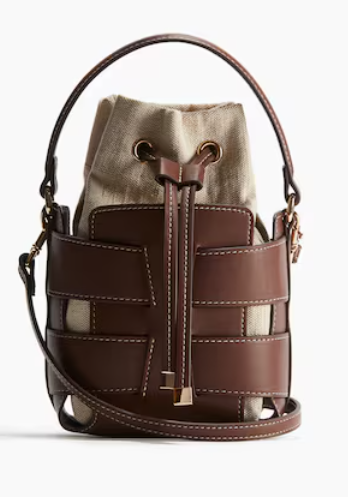
\includegraphics[width=2.5cm,clip,keepaspectratio]{005bd619f6044a40bbfb9806716ac2a7.png}
\end{textblock*}

% ---------- En-tête ---------------------------------------------
\begin{center}
  {\fontsize{44pt}{24pt}\selectfont\bfseries Judikael Mourouvin}

  \bigskip
  {\Large Alternant en marketing digital et support informatique}

  \bigskip\bigskip
  \faMapMarker~Route de COCOYER\ 97190 Gosier
  \quad\faEnvelope~\href{mailto:jkmou971@gmail.com}{jkmou971@gmail.com}

  \bigskip
  % Badge LinkedIn (retirez-le si inutile)
  
\begin{tikzpicture}
    \node[draw,fill=white,rounded corners=9pt,inner xsep=8pt,inner ysep=4pt]
         {\color{black}\faLinkedin\ \href{}{}};
  \end{tikzpicture}

  \vspace{-0.3cm}
  \fullrule
\end{center}

% ---------- Profil ----------------------------------------------
\cvsection{Profil}
Professionnel passionné par l’informatique et le marketing digital, je maîtrise la configuration de postes, la maintenance et le diagnostic d’incidents. Mon année d’alternance à la DSI de la Mairie du Gosier m’a permis de développer mes compétences en gestion de projets numériques et en support aux utilisateurs. Aujourd’hui, je souhaite m’investir à plein temps pour apporter rigueur et efficacité à vos initiatives digitales. Mon objectif : conjuguer expertise technique et sens du service pour optimiser vos systèmes d’information.

\medskip\fullrule

% ---------- Expérience ------------------------------------------
\cvsection{Expérience}

\colorbox{maincolor}{%
  \begin{minipage}{\linewidth}
    \textbf{Alternant en Marketing Digital} \\ Mairie du Gosier - DSI \\ 2023-2024
    \begin{itemize}
      \item Coordonné des projets numériques pour optimiser les services municipaux. \item Analysé les besoins des utilisateurs et déployé des solutions adaptées. \item Assuré le support technique et formé les agents aux outils digitaux.
    \end{itemize}
  \end{minipage}}

\vspace{3mm}


\colorbox{maincolor}{%
  \begin{minipage}{\linewidth}
    \textbf{Animateur de la zone informatique} \\ Pôle Emploi, Gosier \\ 2022-2023
    \begin{itemize}
      \item Réalisé l’assistance et le support technique auprès des demandeurs d’emploi. \item Installé, configuré et entretenu les postes de travail de l’espace numérique. \item Diagnostiqué et résolu les incidents pour garantir la disponibilité du matériel.
    \end{itemize}
  \end{minipage}}

\vspace{3mm}


\colorbox{maincolor}{%
  \begin{minipage}{\linewidth}
    \textbf{Stagiaire Informaticien} \\ Numerika, Baie-Mahault \\ 2020-2021
    \begin{itemize}
      \item Configuré et maintenu les équipements informatiques de l’entreprise. \item Apporté un support de proximité aux utilisateurs pour leurs problématiques quotidiennes.
    \end{itemize}
  \end{minipage}}

\medskip\fullrule

% ---------- Éducation -------------------------------------------
\cvsection{Éducation}

    \begin{tabularx}{\linewidth}{@{}c >{\RaggedRight\arraybackslash}X@{}}
    \textcolor{sidetext}{\faGraduationCap} &
    \textbf{Bachelor Marketing Digital} \\
    & CFA IUTS \\
    & \textit{2023-2024} \\
    \end{tabularx}
    \begin{itemize}[leftmargin=*]
  \item Approche stratégique du marketing sur les canaux numériques.
  \item Utilisation d’outils d’analyse de trafic et de gestion de contenu.
\end{itemize}
\vspace{3mm}

    \begin{tabularx}{\linewidth}{@{}c >{\RaggedRight\arraybackslash}X@{}}
    \textcolor{sidetext}{\faGraduationCap} &
    \textbf{BTS Système Numérique option Informatique et Réseaux} \\
    & Lycée de Chevalier Saint Georges, Abymes \\
    & \textit{2019-2021} \\
    \end{tabularx}
    \begin{itemize}[leftmargin=*]
  \item Administration des réseaux et gestion des systèmes informatiques.
  \item Travaux pratiques en maintenance matérielle et développement de solutions embarquées.
\end{itemize}

\medskip\fullrule

% ---------- Compétences -----------------------------------------
\cvsection{Compétences}
\begin{tabular}{@{}p{0.25\linewidth}p{0.18\linewidth}p{0.18\linewidth}p{0.18\linewidth}}\cicon Administration & \cicon Réseaux & \cicon Support & \cicon Maintenance \\
\cicon Diagnostic & \cicon Marketing & \cicon Digital & \cicon Configuration \\
\cicon Assistance & \cicon Formation & ~ & ~ \\\end{tabular}   % grille 3 lignes × 4 colonnes

\end{document}
